% Author: Izaak Neutelings (June, 2018)
\documentclass[border=3pt,tikz]{standalone}
\usepackage{ifthen}
\usepackage{siunitx}
\usepackage{tikz}
\usetikzlibrary{hobby} % for ..
\usetikzlibrary{arrows.meta} % to control arrow size
\tikzset{>={Latex[length=4,width=4]}} % for LaTeX arrow head
\usetikzlibrary{calc,intersections,decorations.markings}
\usepackage{siunitx}
\usepackage{xcolor} % for colored text

\colorlet{mylightblue}{blue!20}
\colorlet{myblue}{blue!50!black}
\colorlet{mydarkblue}{blue!30!black}
\colorlet{mylightred}{red!10}
\colorlet{myred}{red!50!black}
\colorlet{mydarkred}{red!60!black}
\colorlet{mydarkgreen}{green!30!black}

%\tikzstyle{midarr}=[decoration={markings,mark=at position 0.5 with {\arrow{stealth}}},postaction={decorate}]
\tikzset{
  midarr/.style={decoration={markings,mark=at position #1 with {\arrow{stealth}}},postaction={decorate}},
  midarr/.default=0.5
}
\def\tick#1#2{\draw[thick] (#1) ++ (#2:0.03*\ymax) --++ (#2-180:0.06*\ymax)}


\begin{document}


% PHASE TRANSITIONS
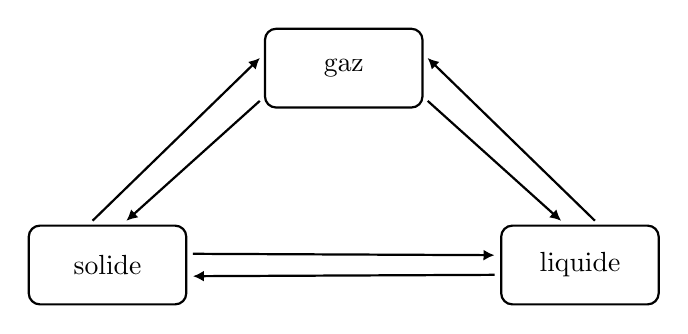
\begin{tikzpicture}[arrow/.style={->,thick,shorten <=2,shorten >=2},
		box/.style={thick,rounded corners=4,inner xsep=6,inner ysep=3}]
	\message{Phase transitions^^J}

	\node[minimum height=1cm, minimum width=2cm, draw, box]
	(S) at (-3,0) {solide};
	\node[minimum height=1cm, minimum width=2cm, draw, box]
	(L) at (3,0) {liquide};
	\node[minimum height=1cm, minimum width=2cm, draw, box]
	(G) at (0,2.5) {gaz};

	\draw[arrow,->] (S.8)
	--
	% to[bend left]
	(L.173) node[above,midway,scale=0.9]
	{};
	\draw[arrow,->]
	(L.-173)
	--
	% to[bend left]
	(S.-8) node[below=-1pt,midway,scale=0.9]
	{};

	\draw[arrow,->]
	(S.115)
	--
	% to[bend left]
	(G.-190)
	node[left=2pt,above,midway,sloped,scale=0.9]
	{};
	\draw[arrow,->]
	(G.-160)
	--
	% to[bend left]
	(S.70)
	node[left=-2pt,below=-1pt,midway,sloped,scale=0.9]
	{};

	\draw[arrow,->]
	(L.65)
	--
	% to[bend left]
	(G.10)
	node[left=2pt,above,midway,sloped,scale=0.9]
	{};
	\draw[arrow,->]
	(G.-20)
	--
	% to[bend left]
	(L.110)
	node[left=2pt,below=-1pt,midway,sloped,scale=0.9]
	{};

\end{tikzpicture}

\end{document}
